\chapter{Réalisation}
\section{Introduction}
Pour faciliter le travail, nous avons utilisé Pyqt5 pour l'implémentation d'une GUI, des modèles pré-formés pour nous aider à obtenir des résultats rapides, et nous avons choisi de former nous-mêmes un modèle "Naive Bayes" sur un ensemble de tweets de 2009 Annexe~\ref{naivebayesimplementation}. L'ensemble de données est composé de plus de 1,6 millions de tweets.
\section{Notre implémenation de Naive Bayes:} 
Pour former notre modèle Bayes naïf, nous importons les données brutes de notre base de données CSV comme suit:\\
\begin{table}[h!]
\centering
    \begin{tabular}{|c|c|} 
    \hline
    score & texte \\ [0.5ex] 
    \hline\hline
    0 & @switchfoot http://twitpic.com/2y1zl - Awww, t... \\ 
    \hline
    0 & is upset that he can't update his Facebook by... \\
    \hline
    0 & @Kenichan I dived many times for the ball. Man... \\
    \hline
    0 & my whole body feels itchy and like its on fire \\
    \hline
    0 & @nationwideclass no, it's not behaving at all.... \\ [0.5ex] 
    \hline
   \end{tabular}
   \caption{Données brutes pour former notre modèle}
   \label{table:1}
\end{table}
Ces tweets bruts doivent être prétraités dans d'autres pour que les Bayes naïfs les utilisent comme un ensemble d'entraînement. Nous ouvrons les tweets chez les pandas pour faciliter la manipulation. Nous choisissons uniquement ce qui nous intéresse dans les colonnes: le texte et la partition.\\

L'ensemble de données est ordonné en deux catégories, positives et négatives. Nous avons donc dû mélanger l'ensemble de données pour créer une distribution aléatoire des entrées et obtenir un ensemble équilibré pour la formation et les tests.\\

Le prétraitement des tweets devait se faire en plusieurs étapes:
\begin{itemize}
    \item Convertir tous les mots en minuscules pour assurer l'homogénéité des tweets et du dictionnaire;
    \item Supprimer les URL et les remplacer par le mot clé "URL" pour préserver l'intégrité des tweets;
    \item Supprimer les marques \@ et les remplacer par le mot-clé "AT\_USER";
    \item Retirez le signe du hashtag;
    \item Tokenize les tweets pour supprimer les caractères répétés puis les diviser en mots;
    \item Tout d'abord, nous avons dû supprimer les mots inutiles basés sur la bibliothèque "stopwords" de NLTK;
\end{itemize}

Après le prétraitement de tous les tweets, nous avons divisé l'ensemble de données en un ensemble d'apprentissage de 95\% de tous les tweets et de 5\% pour le test. \\

Sur la base des tweets traités, nous construisons le dictionnaire de vocabulaire, qui sera utilisé pour faire correspondre les mots avec leur index correspondant, pour permettre au modèle de s'entraîner sur ces index.\\

La formation sur les serveurs Tensor Processing Unit sur Google Colab se bloquait si nous utilisions plus de 100 000 tweets. Nous avons donc opté pour la formation du modèle sur 5000 tweets de base afin de permettre au serveur de gérer le mot et de ne pas prendre plus de 6 heures.

Nous avons obtenu un résultat respectable pour les paramètres par défaut avec une précision de 84\%.\\

Nous enregistrons les poids et les paramètres du modèle à l'aide de cornichons (pickles) et du vocabulaire dans un fichier CSV utilisé pour la prochaine utilisation.
\section{Librairies et APIs utilisés:}
\subsection{Python-Twitter:}
C'est une bibliothèque qui fournit une interface Python pure pour l'API Twitter. Twitter met en disposition un service qui permet aux gens de se connecter via le Web, la messagerie instantanée et les SMS, Twitter expose alors une API Web et cette bibliothèque a pour but de la rendre encore plus facile à utiliser pour les programmeurs Python.\cite{py-twitter}
\subsubsection{Twitter API:}
À un niveau élevé, les API sont la façon dont les programmes informatiques se «parlent» les uns aux autres pour pouvoir demander et fournir des informations. Pour ce faire, une application logicielle peut appeler ce que l'on appelle un point de terminaison:
une adresse qui correspond à un type spécifique d'informations fournis (les points de terminaison (endpoints) sont généralement uniques comme les numéros de téléphone).
Twitter permet d'accéder à certaines parties de l'API pour permettre aux utilisateurs de créer un logiciel qui s'intègre à Twitter.\cite{twitterAPI} \\

Les données Twitter sont uniques par rapport aux données partagées par la plupart des autres plateformes sociales car elles reflètent les informations que les utilisateurs choisissent de partager publiquement, et cet API nous donne l'accès à ces données.
L'API prend également en charge les API qui permettent aux utilisateurs de gérer leurs propres informations Twitter non publiques (par exemple, les messages directs) et de fournir ces informations aux développeurs qu'ils ont autorisés à le faire.
\paragraph{Accéder aux données Twitter:} 
Par défaut, les applications ne peuvent accéder qu'aux informations publiques sur Twitter. Certains points de terminaison (endpoints), tels que ceux chargés d'envoyer ou de recevoir des messages directs, nécessitent des autorisations supplémentaires de la part de l'utilisateur avant de pouvoir accéder à ses informations, et ces autorisations ne sont pas accordées par défaut. \\

L'API Twitter inclut un large éventail de points de terminaison, qui se répartissent en cinq groupes principaux:
\begin{itemize}
    \item \textcolor{DispositionColor}{Comptes et utilisateurs:} L'API permet aux développeurs de gérer (par programme) le profil et les paramètres d'un compte, de désactiver ou de bloquer les utilisateurs, de gérer les utilisateurs et les abonnés, de demander des informations sur l'activité d'un compte autorisé, et d'autres fonctionnalités.
    \item \textcolor{DispositionColor}{Tweets et réponses:} L'API met les Tweets et les réponses publiques à la disposition des développeurs et permet à ces derniers de publier des Tweets. Les développeurs peuvent accéder aux Tweets en recherchant des mots clés spécifiques ou en demandant un échantillon de Tweets à des comptes spécifiques.
    \item \textcolor{DispositionColor}{Messages directs:} Les points de terminaison de message direct permettent d'accéder aux conversations DM des utilisateurs qui ont explicitement accordé l'autorisation à une application spécifique, ils fournissent un accès limité aux développeurs pour créer des expériences personnalisées sur Twitter. Par exemple pour les comptes qu'elles possèdent ou gèrent, les entreprises peuvent créer ces expériences conversationnelles alimentées par des humains ou des "chatbots" pour communiquer directement avec les clients.
    \item \textcolor{DispositionColor}{Les publicités:} Twitter met à disposition une suite d'API pour permettre aux développeurs d'aider les entreprises à créer et gérer automatiquement des campagnes publicitaires sur Twitter. Les développeurs peuvent utiliser des Tweets publics pour identifier les sujets et les intérêts, et fournir aux entreprises des outils pour lancer des campagnes publicitaires pour atteindre les divers publics sur Twitter.
    \item \textcolor{DispositionColor}{Outils de l'éditeur et SDK:} L'API fournit aussi des outils aux développeurs et éditeurs de logiciels pour intégrer des boutons de partage et d'autres contenus Twitter sur des pages Web. Ces outils permettent aux développeurs d'intégrer des conversations publiques en direct de Twitter dans leurs plateformes et facilitent le partage d'informations et d'articles de leurs sites avec les utilisateurs.
\end{itemize}
\subsection{NLTK:}
NLTK (Natural Language Toolkit) est une plate-forme leader pour la construction de programmes Python pour travailler avec des données de langage humain. Il fournit des interfaces faciles à utiliser à plus de 50 corpus et ressources lexicales telles que WordNet, ainsi qu'une suite de bibliothèques de traitement de texte pour la classification, la tokenisation, le stemming, le balisage, l'analyse et le raisonnement sémantique. En autre mot, NLTK aide la machine à analyser, prétraiter et comprendre le texte écrit.\cite{bird2009natural}
\subsubsection{Tokenization:}
"Tokenization" est la première étape de l'analyse de texte. Le processus de décomposition d'un paragraphe de texte en morceaux plus petits tels que des mots ou des phrases est appelé "Tokenization". Le jeton (token) est une entité unique qui constitue des blocs de construction pour une phrase ou un paragraphe.
\subsubsection{Distribution de fréquence:}
NLTK nous permet aussi à calculer la fréquence correspondante à chaque mot donné.
\begin{figure}[H]
    \centering
    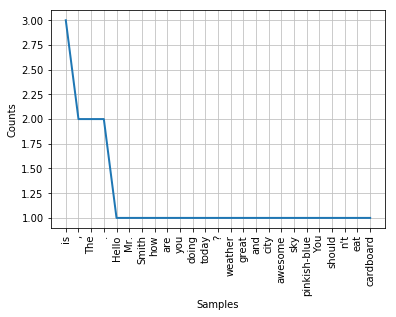
\includegraphics[width=0.8\textwidth]{chapitre3/assets/nltk-freq.png}
    \caption{Exemple d'une représentation de la distribution de fréquence}
    \label{fig:my_label}
\end{figure}
\subsubsection{Mots vides (Stopwords):}
Pour supprimer les mots vides dans NLTK, on doit créer une liste de mots vides et filtrer la liste de jetons à partir de ces mots.
\subsubsection{Normalisation du lexique:}
La normalisation du lexique considère un autre type de bruit dans le texte. Par exemple, "connexion", "connecté", "connectant" se réduit à un mot commun "se connecter". Il réduit les formes dérivées d'un mot à un mot racine commun.
\paragraph{Stemming:}
Le "Stemming" est un processus de normalisation linguistique, qui réduit les mots à leur mot racine ou coupe les affixes de dérivation.
\paragraph{Lemmatisation:}
La lemmatisation réduit les mots à leur mot de base.
\subsubsection{Balisage par catégorie grammaticale (POS tagging):}
L'identification du groupe grammatical d'un mot donné.
\begin{figure}[H]
    \centering
    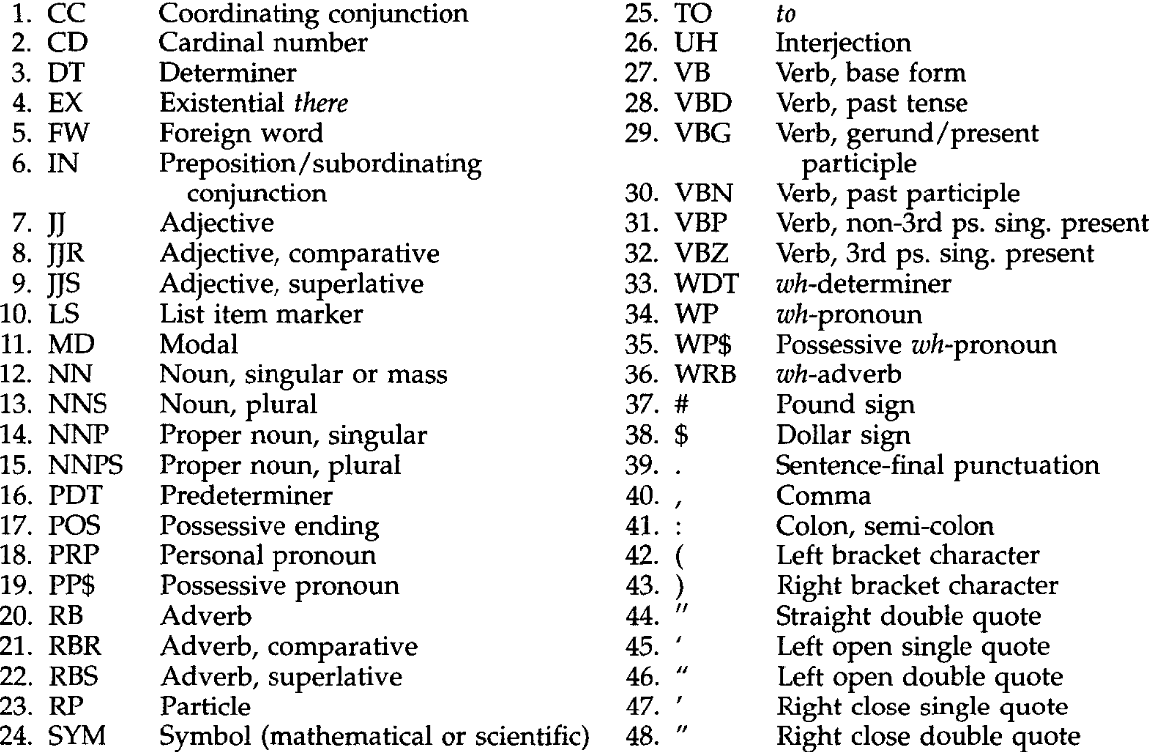
\includegraphics[width=\textwidth]{chapitre3/assets/nltk-pos.png}
    \caption{Différents "POS tags" pour la langue anglaise}
    \label{fig:my_label}
\end{figure}
\subsection{TextBlob:}
TextBlob est une bibliothèque Python pour le traitement de données textuelles. Il fournit une API simple pour plonger dans des tâches courantes de traitement du langage naturel (NLP) \cite{loria2018textblob}, il nous permet d'analyser les sentiments d'un texte et classer le résultat en deux catégories:
\begin{itemize}
    \item \textcolor{DispositionColor}{Polarité:} est une valeur flottante dans la plage [-1,0 à 1,0] où 0 indique neutre, +1 indique un sentiment très positif et -1 représente un sentiment très négatif.
    \item \textcolor{DispositionColor}{Subjectivité:} est une valeur flottante dans la plage [0,0 à 1,0] où 0 est très objectif et 1 est très subjectif. La phrase subjective exprime certains sentiments personnels, vues, croyances, opinions, allégations, désirs, croyances, soupçons et spéculations alors que les phrases objectives sont factuelles.
\end{itemize}
TextBlob est en fait construit sur NLTK et Pattern (un autre module de traitement de données textuelles), il fournit une interface facile à utiliser à la bibliothèque NLTK, et nous permet donc d'utiliser une variété de fonctionnalités telles que le balisage par catégorie grammaticale (POS tagging), "Tokenization", "Stemming", Lemmatisation et bien d'autres:
\subsubsection{Convertir le texte au singulier et au pluriel:}
Quand on passe le texte qu'on veut analyser comme paramètre à la classe "TextBlob", TextBlob nous permet de convertir l'objet retourné au singulier ou au pluriel à l'aide de deux méthode: "singularize()" et "pluralize()".
\subsubsection{Extraction de phrases nominales:}
L'extraction de phrases nominales, comme son nom l'indique, fait référence à l'extraction de phrases débutant avec des noms. Pour le faire on doit simplement utiliser les attributs "noun\_phrase" sur l'objet TextBlob.
\subsubsection{Correction d'orthographe:}
La correction d'orthographe est l'une des fonctionnalités uniques de TextBlob. Avec la méthode "correct()" de l'objet TextBlob, on peut corriger toutes les fautes d'orthographe dans votre texte.
\subsubsection{Traduction de la langue:}
L'une des capacités les plus puissantes de TextBlob est de traduire d'une langue à une autre. Sur le backend, le traducteur de langue TextBlob utilise l'API Google Translate. Il suffit de passer le texte à l'objet TextBlob puis d'appeler la méthode "translate" sur l'objet. Le code de langue souhaitée comme résultat est transmis en tant que paramètre à la méthode.
On peut même détecter la langue d'une phrase en utilisant la méthode "detect\_language()".
\subsubsection{Classification de texte}
TextBlob fournit également des capacités de classification de texte de base. Cependant, TextBlob n'est pas recommandé pour la classification de texte pour les modèles avancés en raison de ses capacités limitées, c'est mieux donc d'utiliser des bibliothèques d'apprentissage automatique telles que Scikit-Learn ou Tensorflow.
\section{Interface graphique}
Pour l'interaction du client avec notre système, nous avons choisi d'utiliser Pyqt5 pour implémenter une GUI simple et intuitive composée de deux fenêtres:
\begin{figure}[H]
    \centering
    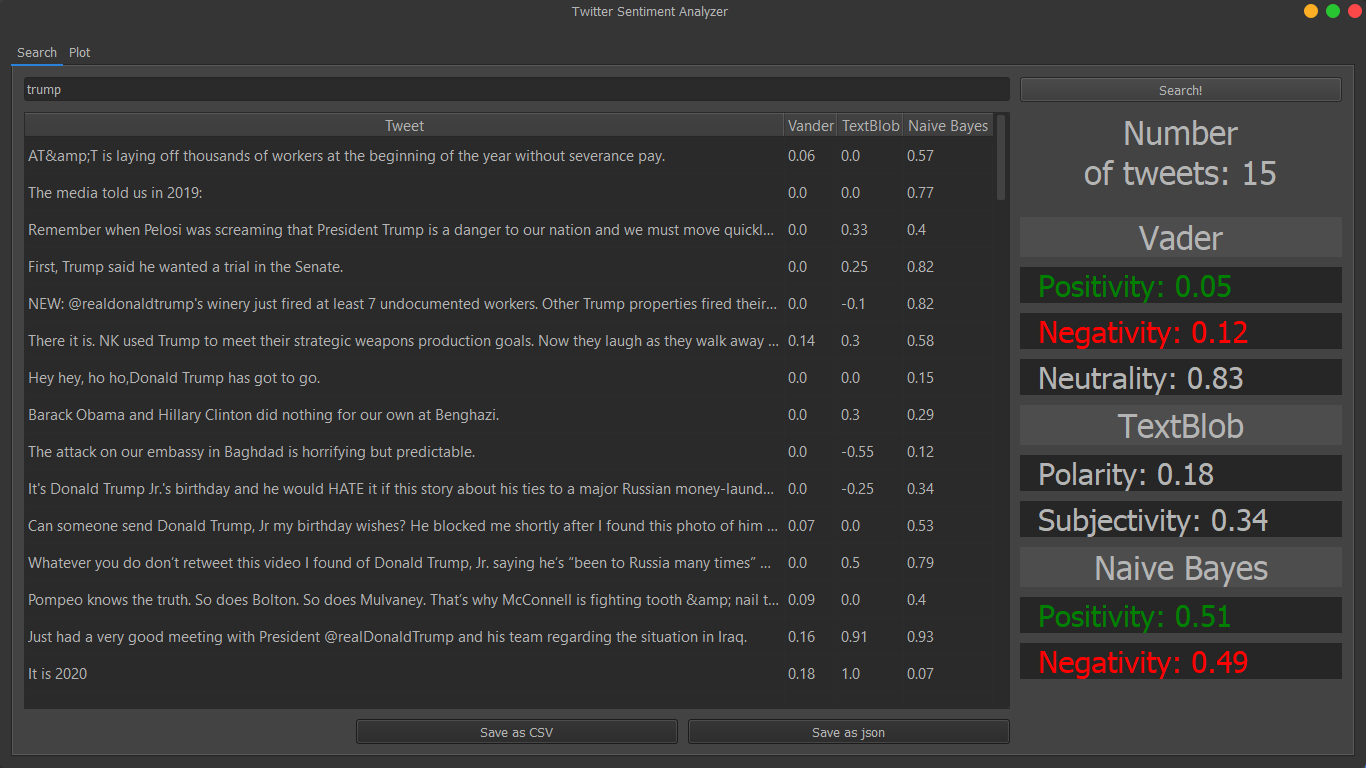
\includegraphics[width=\textwidth]{realisation/assets/1.png}
    \caption{fenêtre de recherche}
    \label{fig:my_label}
\end{figure}
Comme on voit dans la photo ci-dessus, la fenêtre de recherche donne la possibilité au client de:
\begin{itemize}
    \item Entrer un mot ou une phrase et rechercher (en cliquant sur "search") les tweets qui contiennent le texte entré.
    \item Visionner le nombre total et les résultats de ces tweets, les scores de chaque tweet, et le score moyen de tous les tweets selon les différents outils d'analyse de sentiments utilisés.
    \item Enregistrer ses résultats dans le disque dur selon le format choisi (Save as CSV, Save as JSON) 
\end{itemize}
\begin{figure}[H]
    \centering
    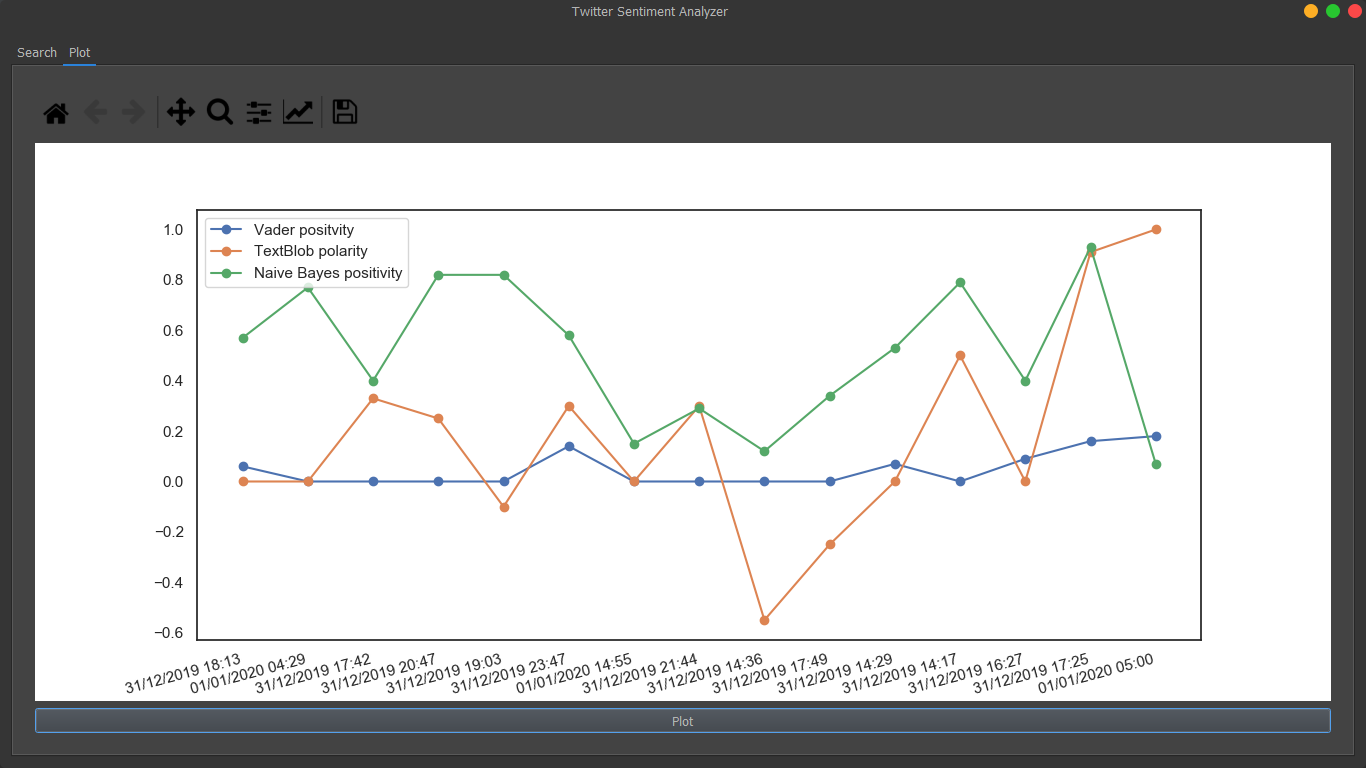
\includegraphics[width=\textwidth]{realisation/assets/2.png}
    \caption{fenêtre de graphe}
    \label{fig:my_label}
\end{figure}
La fenêtre "plot" donne la main au client pour:
\begin{itemize}
    \item Tracer graphiquement (en cliquant sur "plot") les variations de sentiments selon les moyens d'analyse de sentiments présents.
    \item Enregistrer ces graphes dans le disque dur (en cliquant sur l'icone d'enregistrement).
\end{itemize}
\section{Conclusion}
Dans ce chapitre, nous avons détaillé notre implémentation de l'algorithme Bayes Naive, discuté les différentes librairies et APIs choisis pour la réalisation du projet, aussi que les différents écran constituant notre interface graphique.
